\documentclass[conference]{IEEEtran}
\usepackage{cite}
\usepackage[utf8x]{inputenc}
\usepackage{amsmath,amssymb,amsfonts}
\usepackage{algorithmic}
\usepackage{graphicx}
\usepackage{textcomp}
\usepackage[table]{xcolor}
\usepackage{float}
\usepackage[caption=false]{subfig}
\def\BibTeX{{\rm B\kern-.05em{\sc i\kern-.025em b}\kern-.08em
    T\kern-.1667em\lower.7ex\hbox{E}\kern-.125emX}}
\begin{document}

\title{Traversability Learning from Aerial Images with Fully Convolutional Neural Networks\\
% {\footnotesize \textsuperscript{*}Note: Sub-titles are not captured in Xplore and
% should not be used}
% \thanks{Identify applicable funding agency here. If none, delete this.}
}

\author{\IEEEauthorblockN{Borges, C. D. B}
\IEEEauthorblockA{\textit{Programa de Pós-Graduação em Engenharia Elétrica e de Computação} \\
\textit{Universidade Federal do Ceará -- Campus Sobral}\\
Sobral, Brazil \\
davidborges@protonmail.com}
% \and
% \IEEEauthorblockN{2\textsuperscript{nd} Given Name Surname}
% \IEEEauthorblockA{\textit{dept. name of organization (of Aff.)} \\
% \textit{name of organization (of Aff.)}\\
% City, Country \\
% email address}
% \and
% \IEEEauthorblockN{3\textsuperscript{rd} Given Name Surname}
% \IEEEauthorblockA{\textit{dept. name of organization (of Aff.)} \\
% \textit{name of organization (of Aff.)}\\
% City, Country \\
% email address}
}

\maketitle

\begin{abstract}
Traversability computation is a key step for robot path planning.
It allows the incorporation of knowledge about traversable and non-traversable terrain into the robot's planning algorithms.
It is possible to use aerial data to compute traversability maps for large regions of land and use them to assist ground robot navigation.
Most published methods to generate these maps from aerial images use terrain classification in combination with predefined traversability values for each class or simple heuristics.
Classification, however, can be computationally expensive. 
Using only handcrafted heuristics disregards the possible advantage of learning hidden structures in image data.
This work describes a new method to compute a traversability map from an aerial image in only one forward pass through a fully convolutional neural network.
It analyzes the advantages and current disadvantages of this approach.
The experiments yield evidence that the proposed model can generate traversability maps faster while also providing lower error outputs.
\end{abstract}

\begin{IEEEkeywords}
traversability, mapping, convolutional neural networks, aerial images, ground robot, path planning
\end{IEEEkeywords}

\section{Introduction}

The traversability index was proposed by Seraji \cite{seraji:1999}.
It was a simple way to distinguish traversable from non-traversable terrain and apply this knowledge to navigation strategies for robots.
Traversability is a quantification of how much a given region is suitable to be crossed by a moving robot or vehicle.
The concept was extended and applied in robot planning tasks using a wide range of techniques to estimate traversability maps, from digital images to laser scanning \cite{howard:2001,howard:2003,castejon:2005,guo:2008,shneier:2008}.

With the rise in popularity of low cost multirotor drones and the increased availability of high resolution satellite images, a new idea to assist in robot navigation surfaced: the use of aerial images to add long range planning capabilities to ground robots.
This was explored, for example, by \cite{vandapel:2006,hudjakov:2011,hudjakov:2013,delmerico:2017,borges:2019} and others.
In these works, some of the proposed methods to generate traversability maps require depth data \cite{vandapel:2006,delmerico:2017}, while others need only RGB images \cite{hudjakov:2011,hudjakov:2013,borges:2019}.
The core traversability computation approach also varied between heuristics \cite{vandapel:2006,borges:2019} and classification + heuristics \cite{hudjakov:2011,hudjakov:2013,delmerico:2017}.

This work proposes a machine learning approach to compute traversabilities from raw image data.
It is an extension of the method described in \cite{borges:2019} that replaces the heuristic-based sub-region computations with an end-to-end traversability estimation based on a fully convolutional neural network.
This method is described in detail in section \ref{section:proposed-method}.
The experiments performed to validate the network architecture are explained in section \ref{section:experiments}.
Results and a discussion about the merits and drawbacks of the method are explored in sections \ref{section:results} and \ref{section:discussion}.
Section \ref{section:conclusion} closes this paper with a brief review.

\section{Proposed Method}
\label{section:proposed-method}

The mapping and planning approach previously described in \cite{borges:2019} is shown in Fig. \ref{fig:eswa}.
The input image, which is an aerial view of the ground region, is submitted to bilateral filtering and partitioned into sub-regions that may overlap.
A predefined function is used to compute a degree of traversability for each sub-region.
These values are then stored in a traversability matrix ($\mathcal{T}$) that preserves the relative position of the sub-regions.
$\mathcal{T}$ is used to build a graph representation of the region and its traversabilities; in this graph, vertices represent sub-regions and edge weights are inversely proportional to the traversability between adjacent regions.
A shortest path search algorithm is then used to find a path between any chosen source and target sub-regions.

\begin{figure*}[ht]
\centering

\subfloat[ESWA proposal]{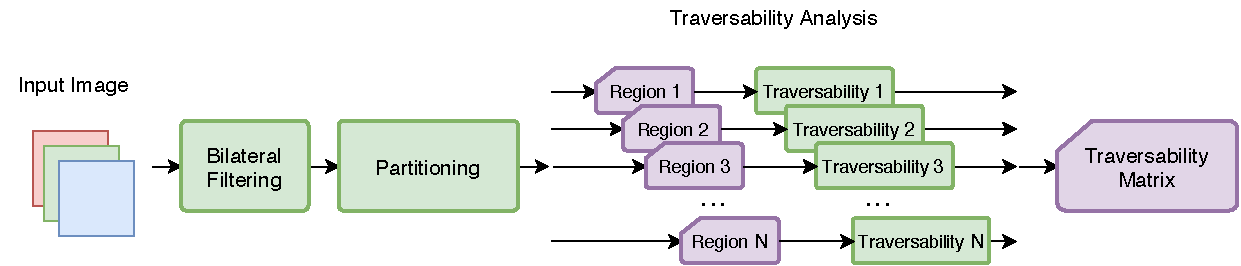
\includegraphics[width=0.75\textwidth]{graphics/eswa-proposal-flowchart.pdf}\label{fig:eswa}}

\vspace{0.75cm}

\subfloat[TFCN proposal]{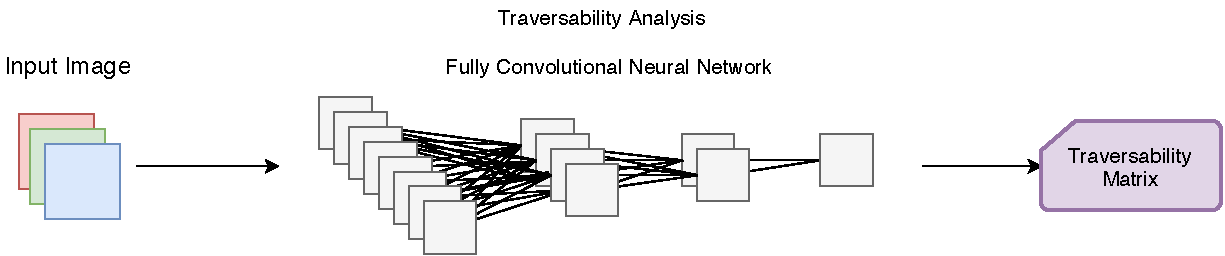
\includegraphics[width=0.75\textwidth]{graphics/proposal-flowchart.pdf}\label{fig:proposal}}

\caption{Experimental results}
\label{fig:flocharts}
\end{figure*}

This work builds upon the approach described in \cite{borges:2019}, replacing the conventional preprocessing, partitioning and traversability computation pipeline with a Fully Convolutional Neural Network (FCN), as displayed in Fig. \ref{fig:proposal}.
The proposed traversability estimation method uses an FCN to derive a traversability matrix $\mathcal{T}$ directly from raw RGB images.
The Traversability FCN (TFCN) architecture is shown in Fig. \ref{fig}.
It is a small network, composed of three phases of convolutions and pooling.
Batch normalization steps are performed after convolutional layers as a way to mitigate internal covariate shift and reduce training time \cite{ioffe:2015}.
In order to counter overfitting, the TFCN also performs dropout \cite{srivastava:2014} and L2 regularization \cite{ng:2004}.

\begin{figure}[htbp]
\centerline{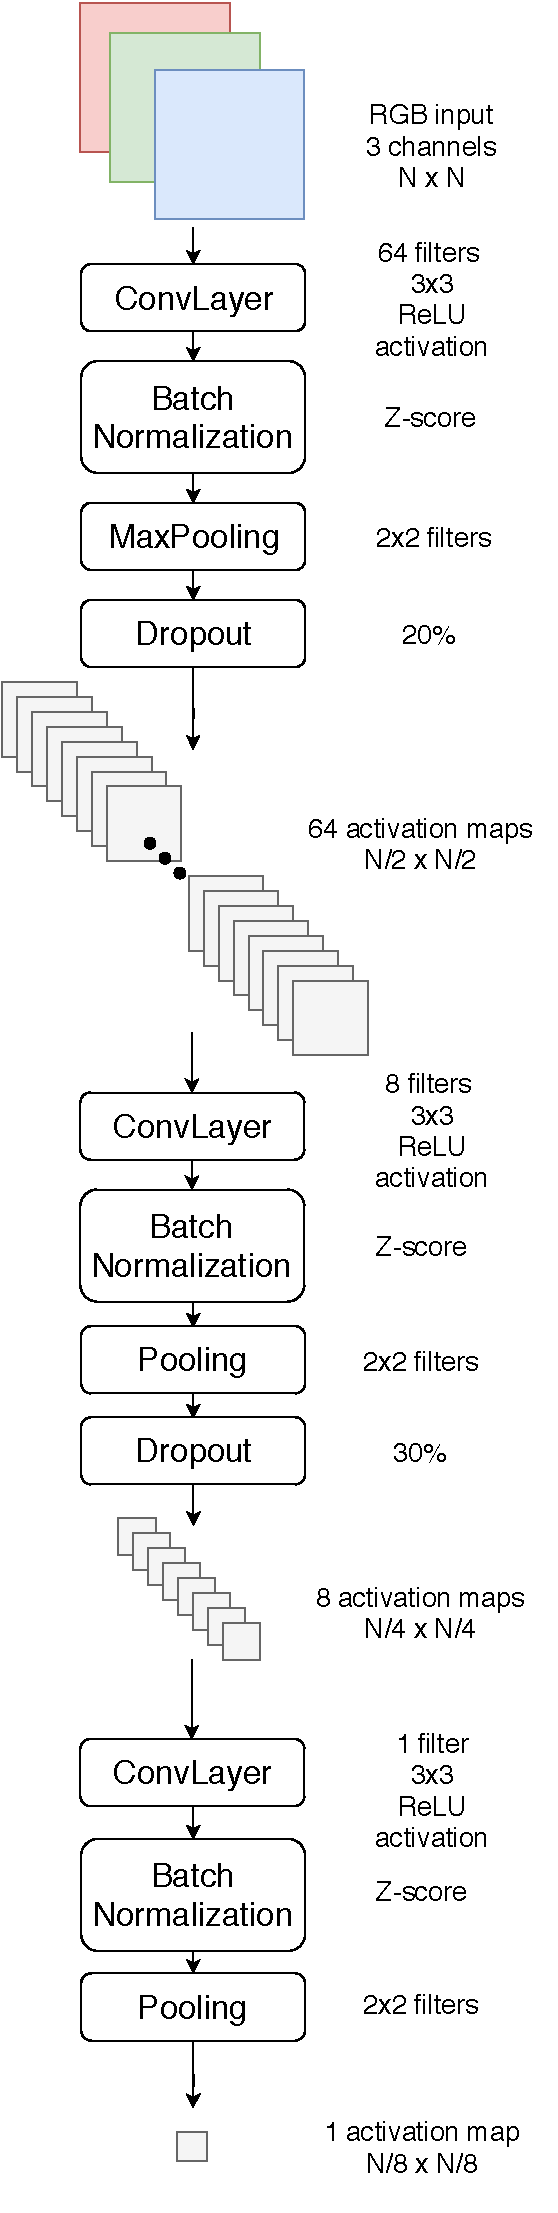
\includegraphics[width=0.3\textwidth]{graphics/TFCN.pdf}}
\caption{Example of a figure caption.}
\label{fig}
\end{figure}

\section{Experiments}
\label{section:experiments}

To validate the new traversability estimation method, the proposed TFCN was trained and tested on the Aerial Traversability and Planning Dataset \cite{borges:2019}.
This section describes ATPD, the training configuration and the cross-validation approach employed in the experiments.

\subsection{Dataset}

The Aerial Traversability and Planning Dataset (ATPD) \cite{borges:2019} contains 8 orthorectified aerial images of size $1000 \times 1000$ pixels, with specified spatial resolutions of about $0.3 \times 0.3 \ m^2/p$.
Each image has a corresponding traversability label, in which every pixel from the original image is assigned a binary value: 1 if the original pixel is in a traversable sub-region and 0 otherwise.
% An aerial image and its traversability label from ATPD can be seen in Fig. \ref{fig:atpd-sample}.
% The dataset also includes two sets of keypoint coordinates for each image. 
% The first set has 12 reachable keypoints (Fig. \ref{fig:positive-keypoints}) and is useful to verify whether a path planning approach can generate a safe route between them.
% The second set has 12 unreachable keypoints (Fig. \ref{fig:negative-keypoints}) and is used to test if a planner is able to detect and avoid impossible paths.

% \begin{figure}[H]
% \centering
% \subfloat[Aerial image. \label{fig:aerial-image}]{
% 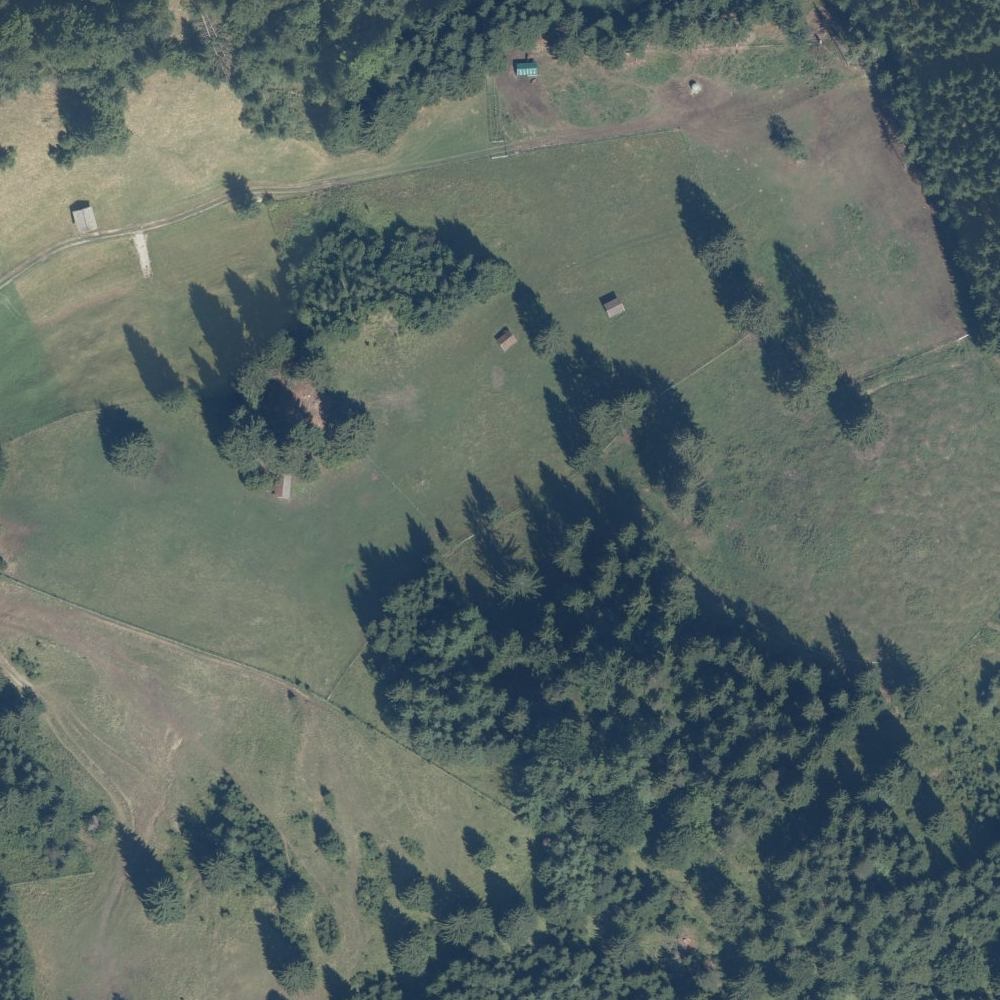
\includegraphics[width=0.23\textwidth]{graphics/aerial07.jpg}
% }
% \hfill
% \subfloat[Binary traversability label. \label{fig:traversability-label}]{%
% 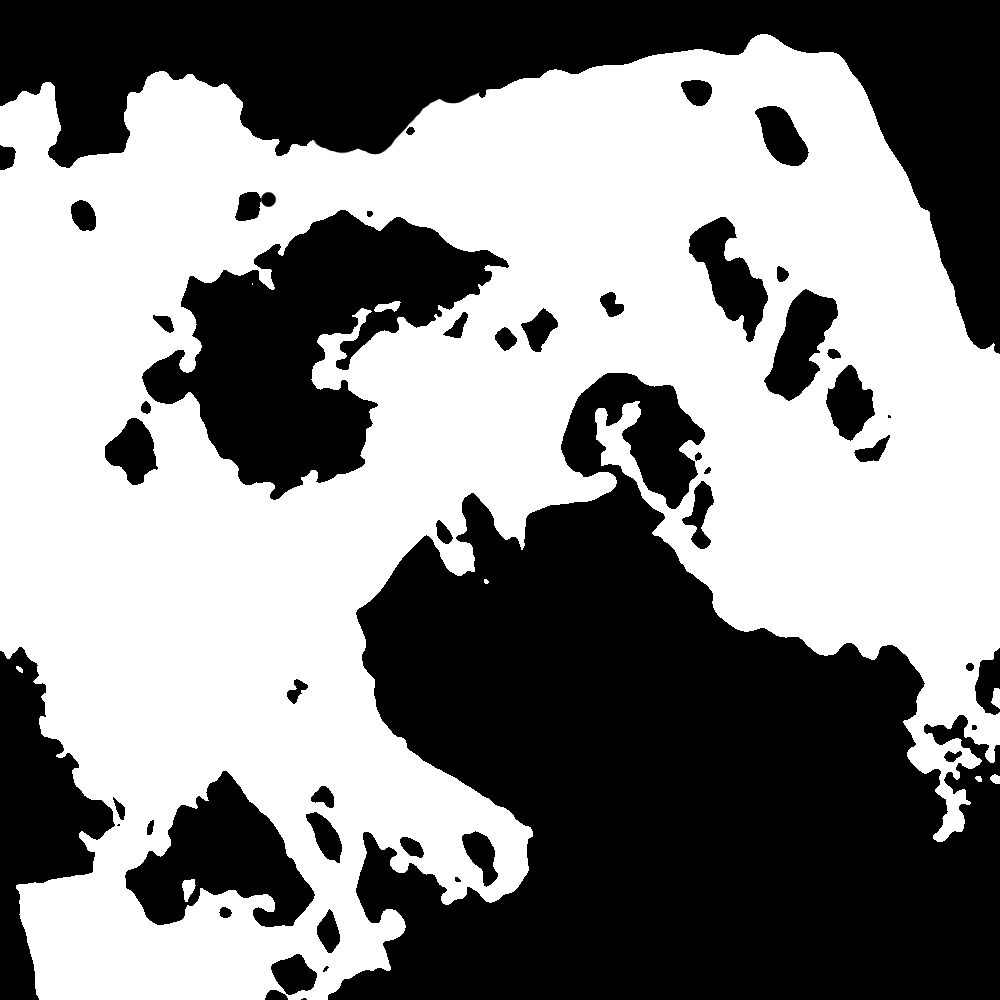
\includegraphics[width=0.23\textwidth]{graphics/aerial07-trav.jpg}
% }

% \subfloat[Reachable keypoints. \label{fig:positive-keypoints}]{
% 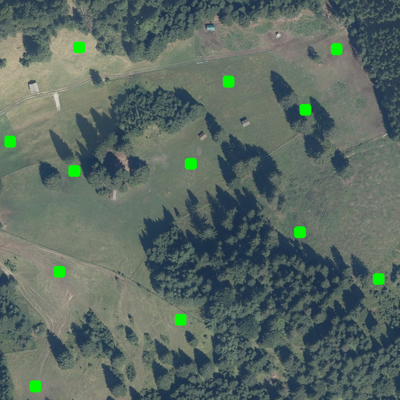
\includegraphics[width=0.23\textwidth]{graphics/aerial07-positive.jpg}
% }
% \hfill
% \subfloat[Unreachable keypoints. \label{fig:negative-keypoints}]{%
% 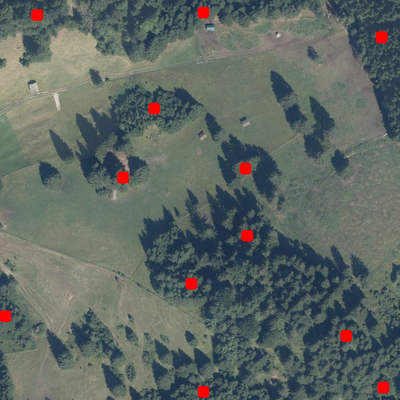
\includegraphics[width=0.23\textwidth]{graphics/aerial07-negative.jpg}
% }
% \caption{A sample from ATPD.}
% \label{fig:atpd-sample}
% \end{figure}

\subsection{Data Augmentation}

It is known that a convolutional neural network (CNN) usually requires a large amount of training data in order to converge and perform properly [needs citation].
However, ATPD only includes 8 aerial images with labeled traversabilities.
It is a very small dataset for a CNN.
For this reason, the training sets are augmented with random rotations, shifts, flips, shear and zoom.
The outcome of these operations might require padding (e.g. rotation, shift and shear).
In these cases, the resulting image is padded by reflection, so that added pixels are similar to those in the neighboring region.

\subsection{Training}

The TFCN was trained with Adam optimization \cite{kingma:2015}, mean squared error (MSE) loss and early stopping \cite{prechelt:2012}.
Training was carried on for a maximum of 100 epochs, but interrupted if there was no validation loss improvement after 20 consecutive epochs.
A checkpoint routine was used to save the weight configuration with the best validation loss during each training execution.
This configuration was the output of the training phase in the experiments.

\subsection{Cross-validation}

An image-based leave-one-out cross-validation was employed to study the generalization capability of the TFCN.
In this approach, each of the eight aerial images from ATPD is used once for testing, while the other seven are selected to train the TFCN.
These seven images are further split into a training set composed of six images and their augmentations; and a validation set of one image and its augmentations.
Training sets have $6 \times 128 = 768$ samples (images $\times$ augmentations), while validation sets have $1 \times 128$ samples.

The chosen cross-validation approach is fair because it guarantees that samples from the test set were not used in any way during training.
Moreover, the best weight configuration is chosen based on the loss computed on the validation set, which also has no intersection with the training and test sets.

\section{Results}
\label{section:results}

The behavior of the training and validation losses, along with visualizations of the test images, test labels and TFCN outputs from each leave-one-out step can be seen in Figs. \ref{fig:results-01} through \ref{fig:results-08}.
Because training was done with early stopping, the number of epochs in each leave-one-out step was variable.
This is shown in the graphs as an abrupt interruption of the loss curves after 20 epochs without validation loss improvement.
The average time to complete one epoch was 28 seconds.

The training, validation and test losses obtained using the best weight configuration in each leave-one-out step, together with the number of epochs to finish the training phases, are summarized in Table \ref{tab:results}.
These losses are the sum of the MSE and the L2 regularization penalties.

\begin{table}[htbp]
\begin{center}
\caption{Results}
\begin{tabular}{|c|c c| c c c|}
\hline
\textbf{Leave-one-out} & \textbf{Total} & \textbf{Best} & \textbf{Training} & \textbf{Validation} & \textbf{Test} \\
% \cline{2-4}
\textbf{Step} & \textbf{Epochs} & \textbf{Epoch} & \textbf{Loss} & \textbf{Loss} & \textbf{Loss} \\
\hline
1 &  100 & 93 & 0.0974 & 0.0949 & 0.1265 \\ %\hline
2 & \ 83 & 63 & 0.1106 & 0.0951 & 0.1199 \\ %\hline
3 & \ 65 & 45 & 0.1103 & 0.0701 & 0.1161 \\ %\hline
4 & \ 57 & 37 & 0.1232 & 0.0589 & 0.1011 \\ %\hline
5 & \ 41 & 23 & 0.1643 & 0.0784 & 0.0712 \\ %\hline
6 & \ 52 & 32 & 0.1336 & 0.0869 & 0.0820 \\ %\hline
7 & \ 45 & 25 & 0.1627 & 0.5474 & 0.2302 \\ %\hline
8 & \ 79 & 59 & 0.0950 & 0.1093 & 0.5137 \\ \hline
\end{tabular}
\label{tab:results}
\end{center}
\end{table}

\begin{figure*}[ht]
\centering
\subfloat[Training and validation losses]{
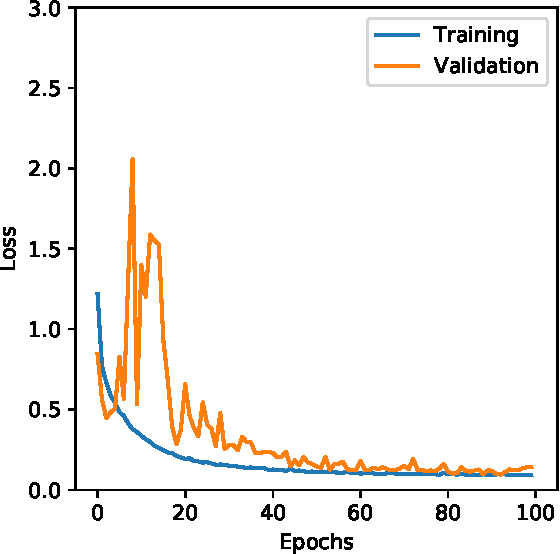
\includegraphics[width=0.23\textwidth]{graphics/loss01.pdf}
\label{fig:results-loss-01}
}
\subfloat[Test image]{
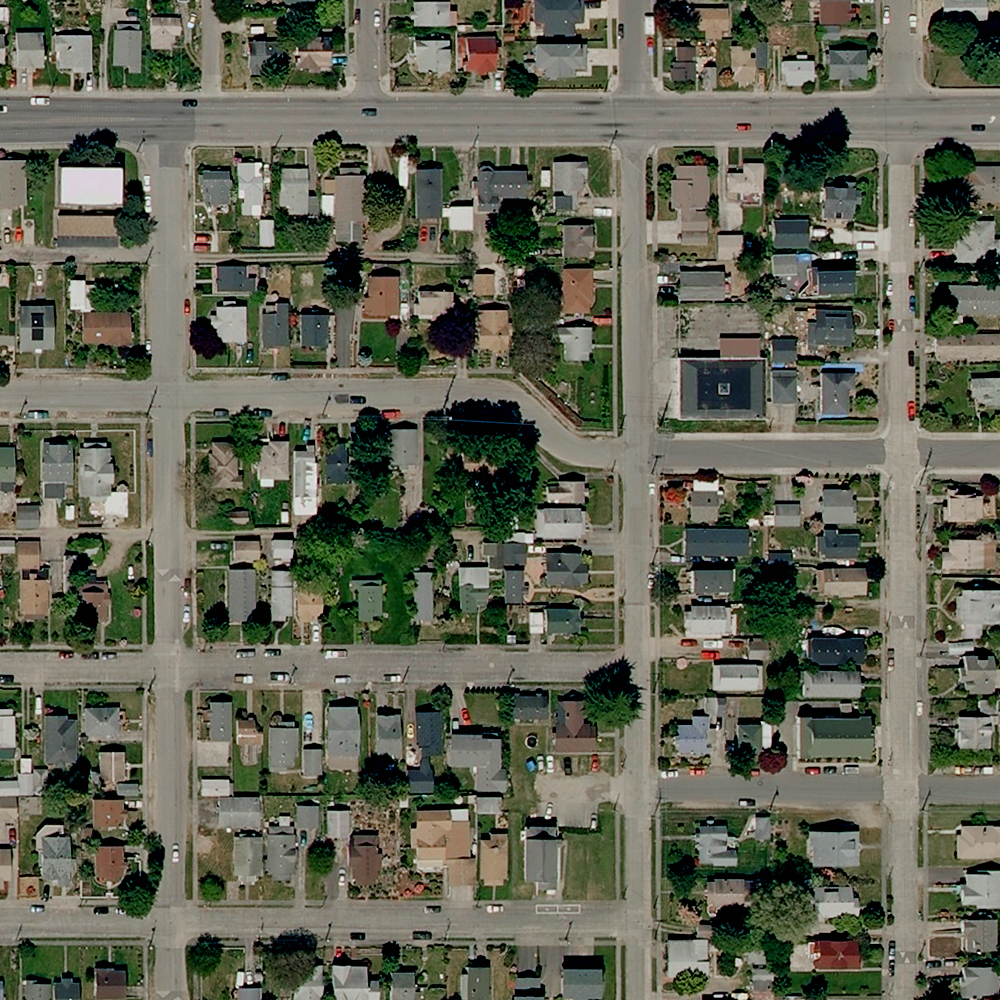
\includegraphics[width=0.23\textwidth]{graphics/aerial01.jpg}
\label{fig:results-input-01}
}
\subfloat[Test label]{
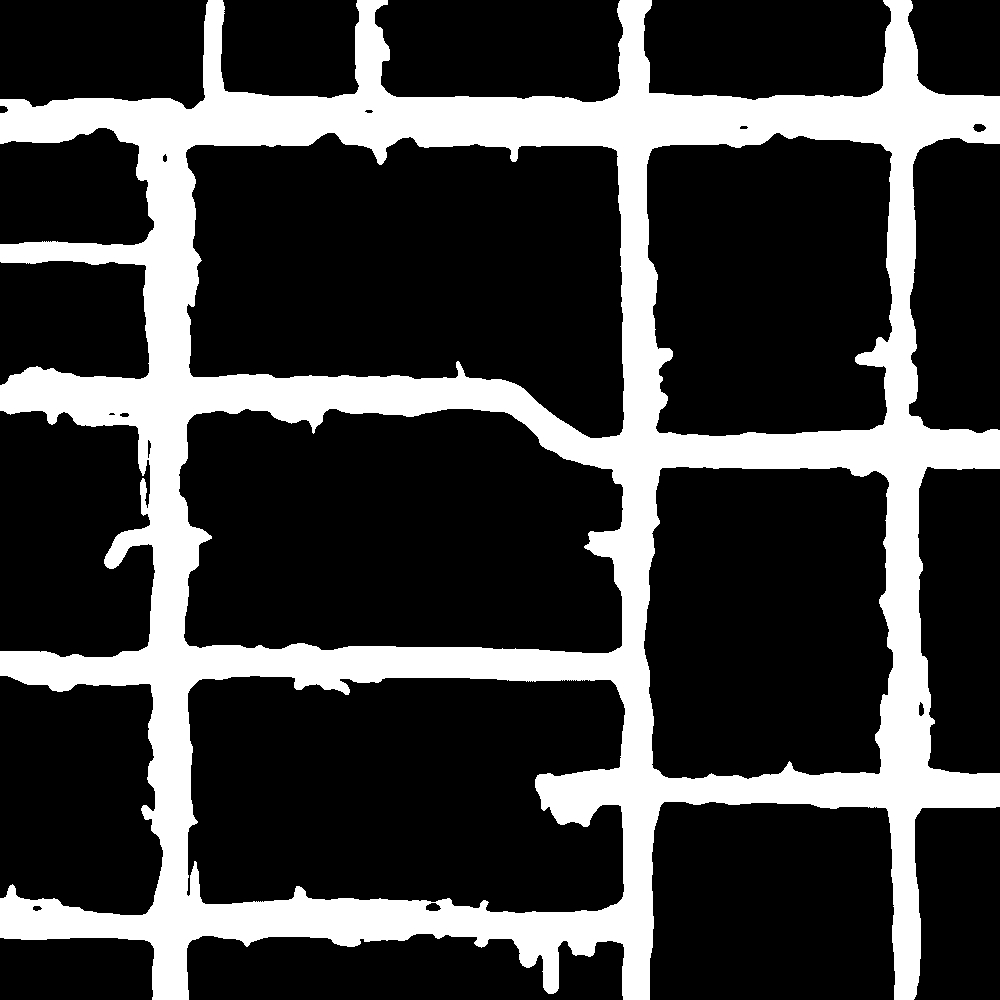
\includegraphics[width=0.23\textwidth]{graphics/aerial01-trav.jpg}
\label{fig:results-trav-01}
}
\subfloat[TFCN output]{
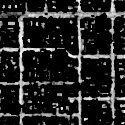
\includegraphics[width=0.23\textwidth]{graphics/tfcn-output-01.jpg}
\label{fig:results-output-01}
}
\caption{Results from cross-validation step 1}
\label{fig:results-01}
\end{figure*}

\begin{figure*}[ht]
\centering
\subfloat[Training and validation losses]{
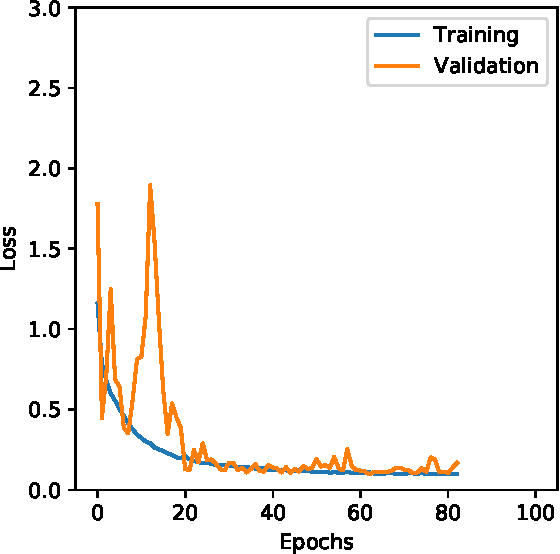
\includegraphics[width=0.23\textwidth]{graphics/loss02.pdf}
\label{fig:results-loss-02}
}
\subfloat[Test image]{
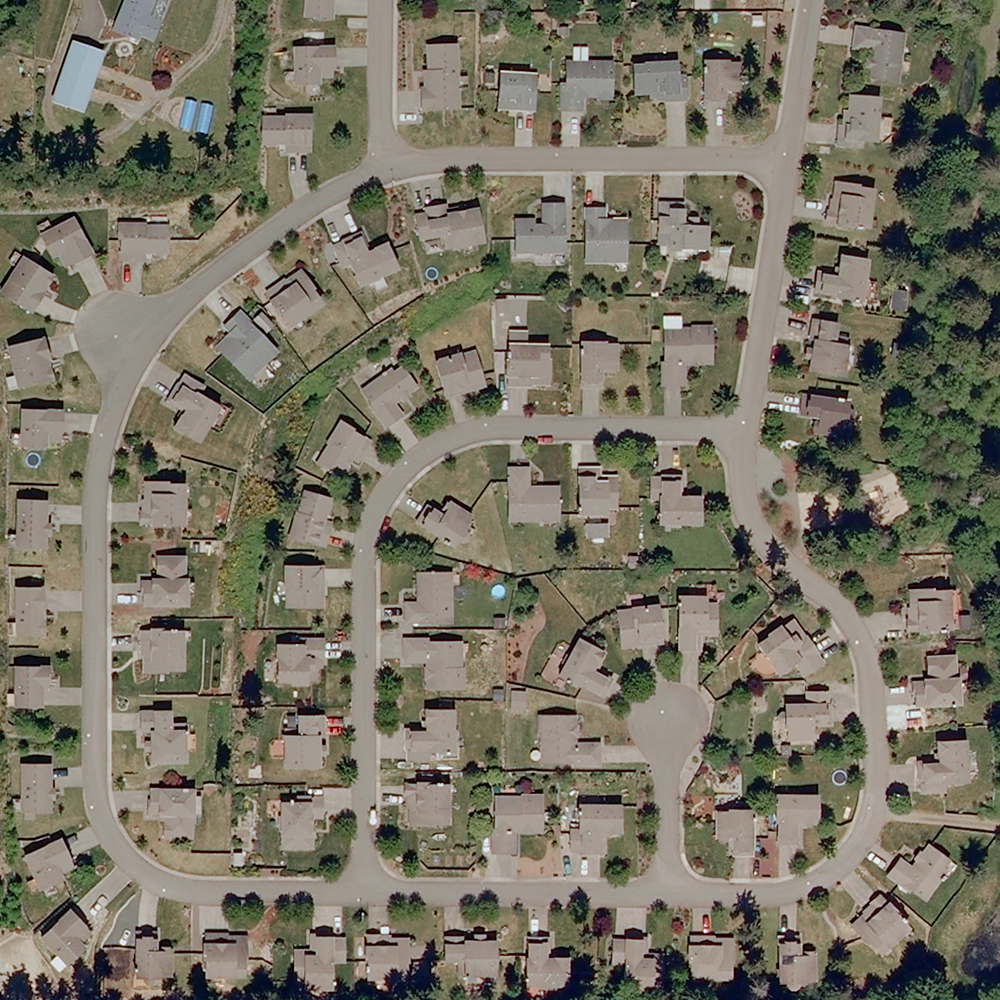
\includegraphics[width=0.23\textwidth]{graphics/aerial02.jpg}
\label{fig:results-input-02}
}
\subfloat[Test label]{

\includegraphics[width=0.23\textwidth]{graphics/aerial02-trav.jpg}
\label{fig:results-trav-02}
}
\subfloat[TFCN output]{
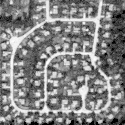
\includegraphics[width=0.23\textwidth]{graphics/tfcn-output-02.jpg}
\label{fig:results-output-02}
}
\caption{Results from cross-validation step 2}
\label{fig:results-02}
\end{figure*}

\begin{figure*}[ht]
\centering
\subfloat[Training and validation losses]{
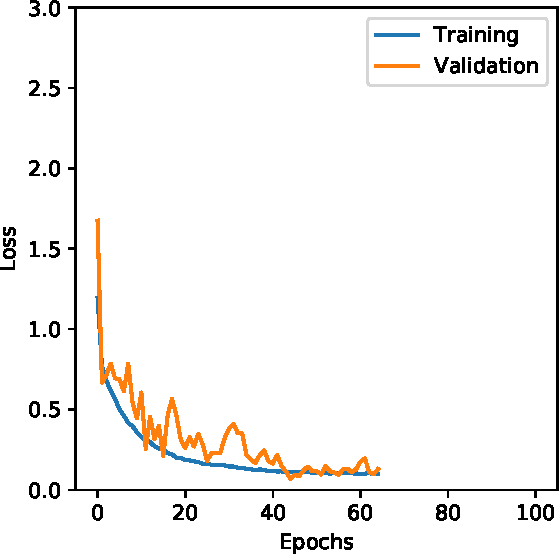
\includegraphics[width=0.23\textwidth]{graphics/loss03.pdf}
\label{fig:results-loss-03}
}
\subfloat[Test image]{
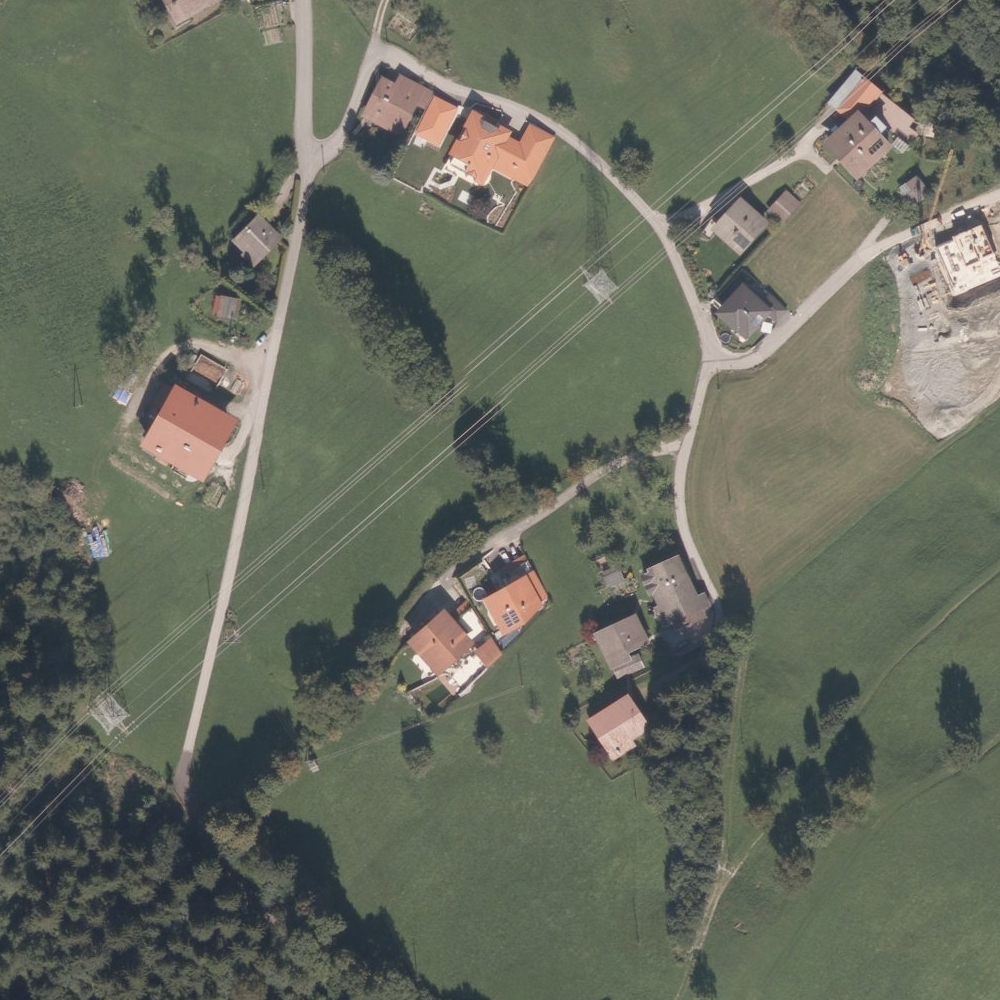
\includegraphics[width=0.23\textwidth]{graphics/aerial03.jpg}
\label{fig:results-input-03}
}
\subfloat[Test label]{
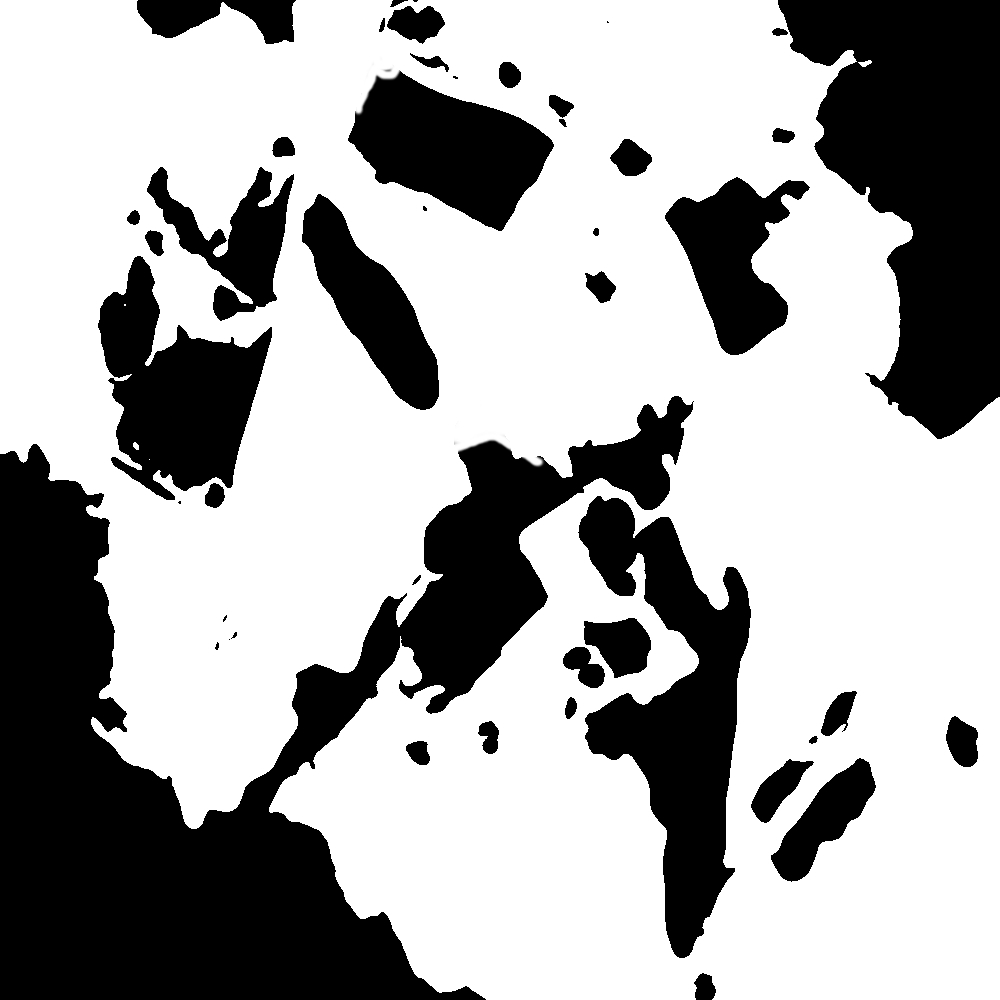
\includegraphics[width=0.23\textwidth]{graphics/aerial03-trav.jpg}
\label{fig:results-trav-03}
}
\subfloat[TFCN output]{
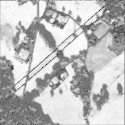
\includegraphics[width=0.23\textwidth]{graphics/tfcn-output-03.jpg}
\label{fig:results-output-03}
}
\caption{Results from cross-validation step 3}
\label{fig:results-03}
\end{figure*}

\begin{figure*}[ht]
\centering
\subfloat[Training and validation losses]{
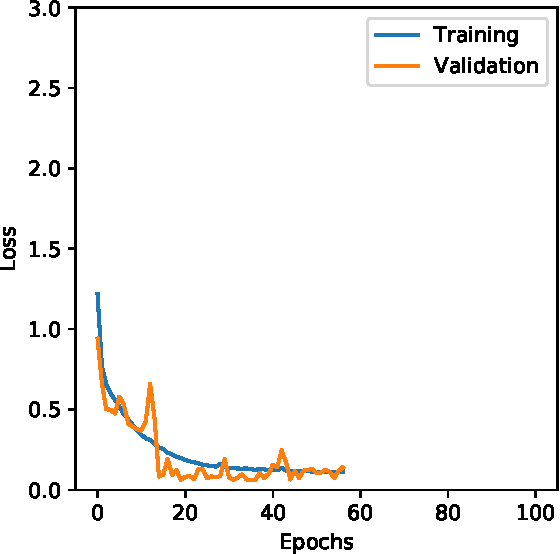
\includegraphics[width=0.23\textwidth]{graphics/loss04.pdf}
\label{fig:results-loss-04}
}
\subfloat[Test image]{
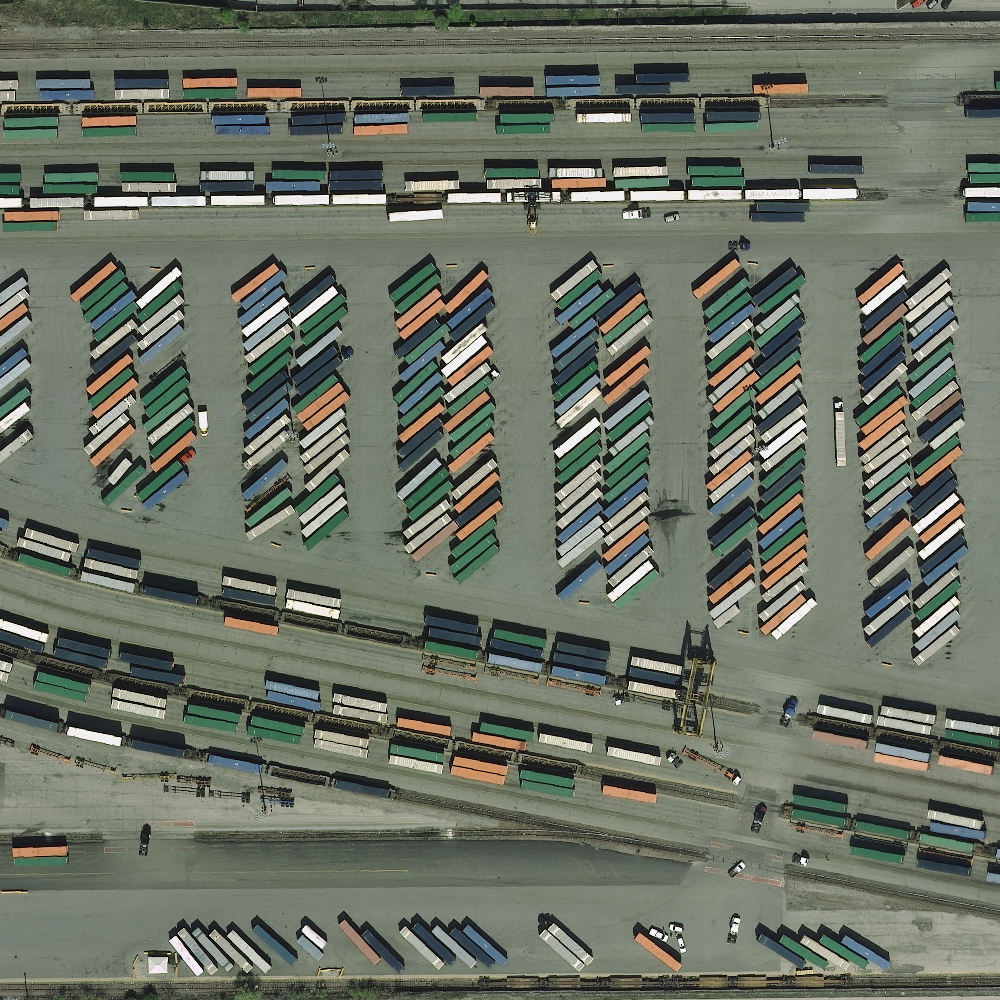
\includegraphics[width=0.23\textwidth]{graphics/aerial04.jpg}
\label{fig:results-input-04}
}
\subfloat[Test label]{
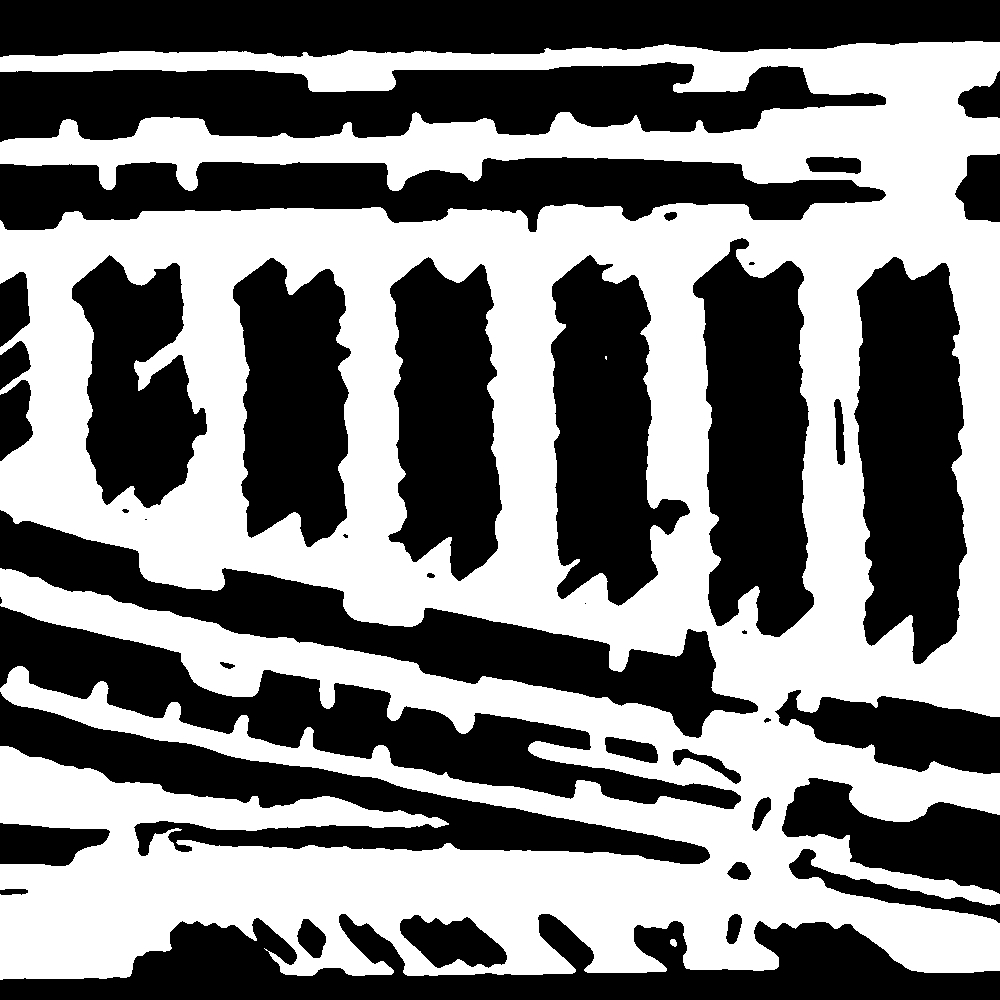
\includegraphics[width=0.23\textwidth]{graphics/aerial04-trav.jpg}
\label{fig:results-trav-04}
}
\subfloat[TFCN output]{
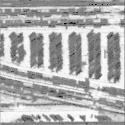
\includegraphics[width=0.23\textwidth]{graphics/tfcn-output-04.jpg}
\label{fig:results-output-04}
}
\caption{Results from cross-validation step 4}
\label{fig:results-04}
\end{figure*}

\begin{figure*}[ht]
\centering
\subfloat[Training and validation losses]{
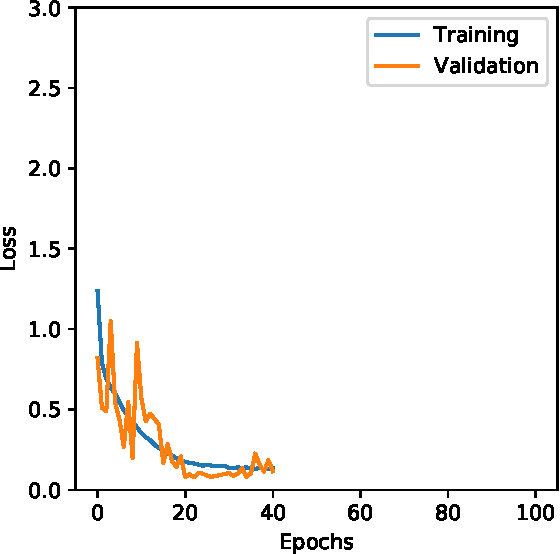
\includegraphics[width=0.23\textwidth]{graphics/loss05.pdf}
\label{fig:results-loss-05}
}
\subfloat[Test image]{
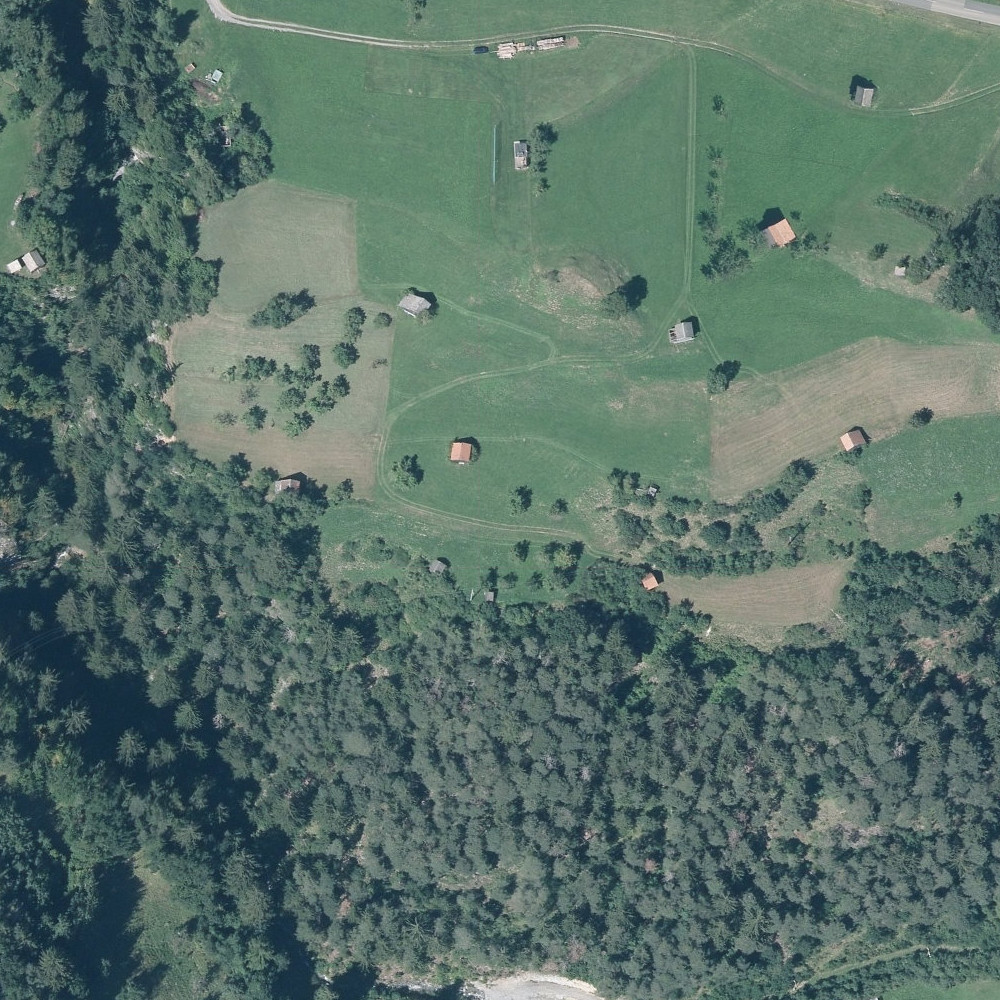
\includegraphics[width=0.23\textwidth]{graphics/aerial05.jpg}
\label{fig:results-input-05}
}
\subfloat[Test label]{
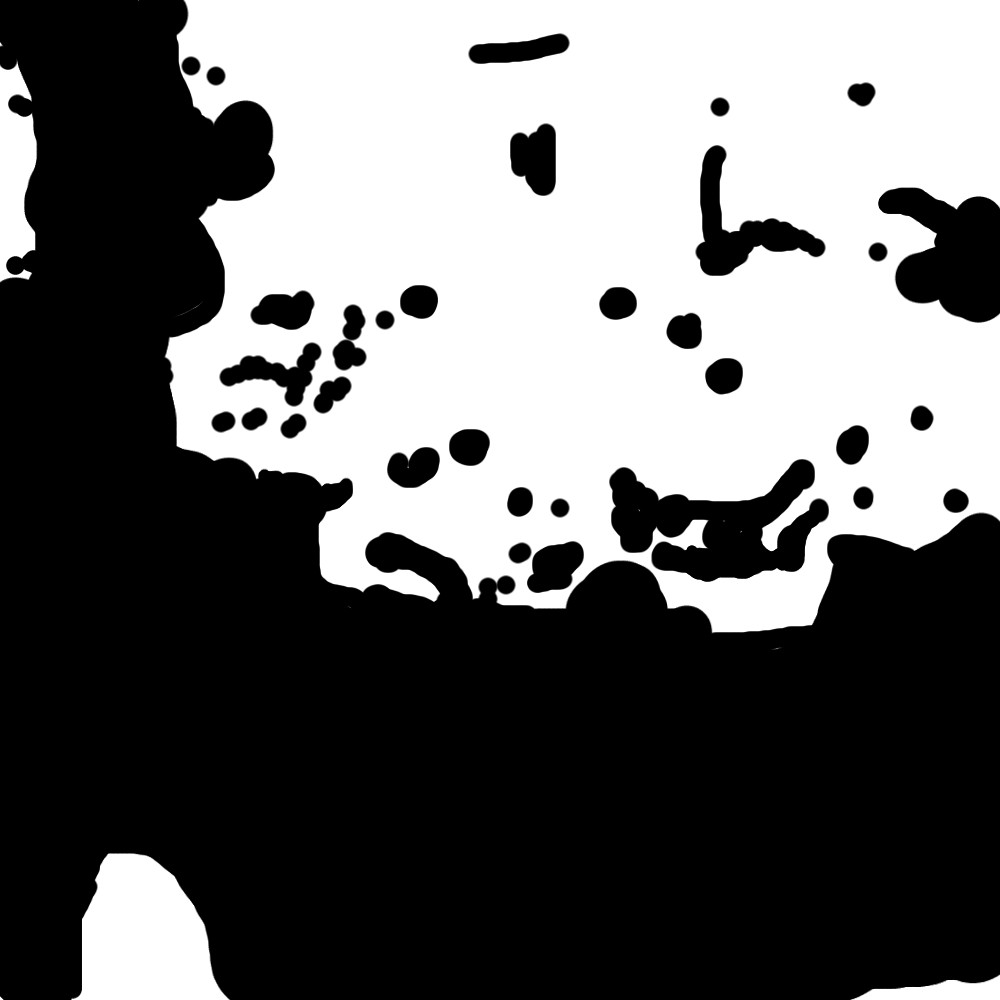
\includegraphics[width=0.23\textwidth]{graphics/aerial05-trav.jpg}
\label{fig:results-trav-05}
}
\subfloat[TFCN output]{
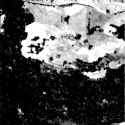
\includegraphics[width=0.23\textwidth]{graphics/tfcn-output-05.jpg}
\label{fig:results-output-05}
}
\caption{Results from cross-validation step 5}
\label{fig:results-05}
\end{figure*}

\begin{figure*}[ht]
\centering
\subfloat[Training and validation losses]{
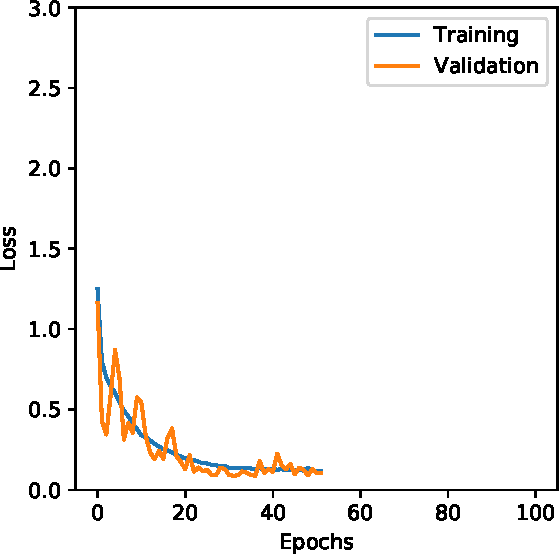
\includegraphics[width=0.23\textwidth]{graphics/loss06.pdf}
\label{fig:results-loss-06}
}
\subfloat[Test image]{
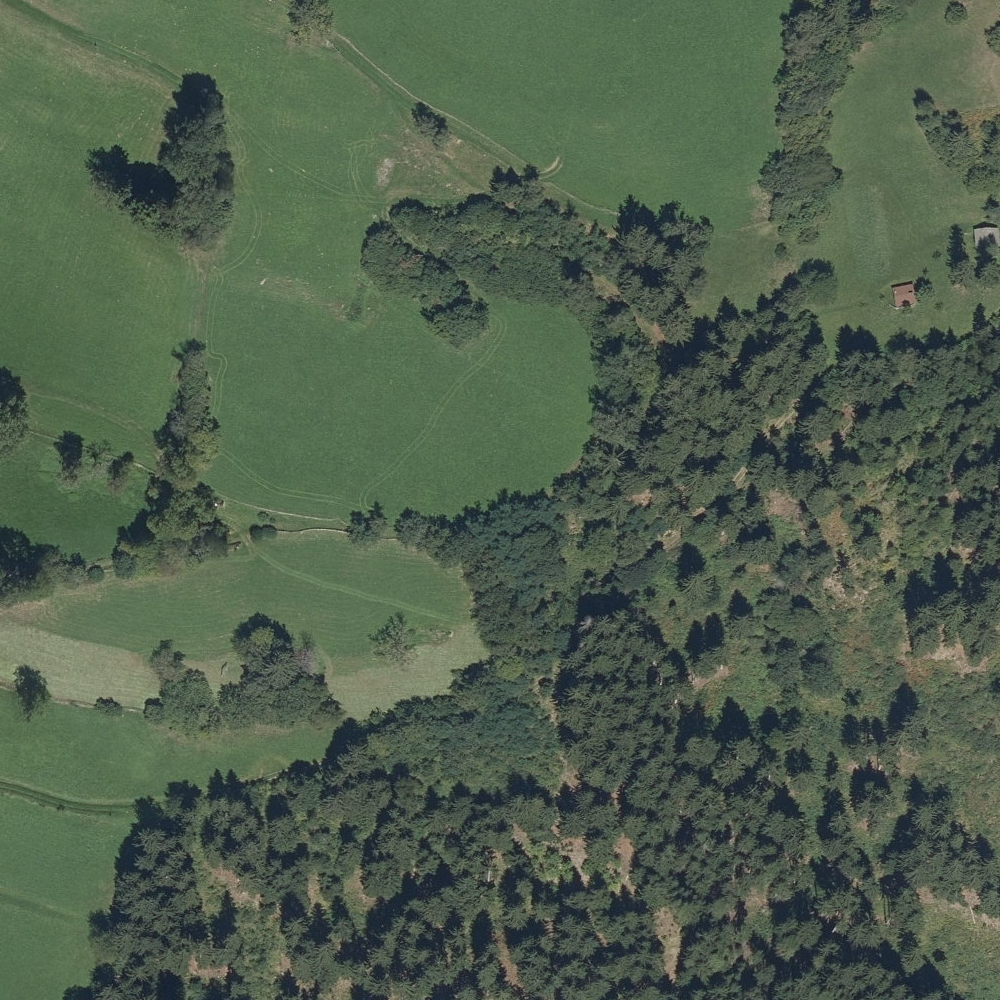
\includegraphics[width=0.23\textwidth]{graphics/aerial06.jpg}
\label{fig:results-input-06}
}
\subfloat[Test label]{
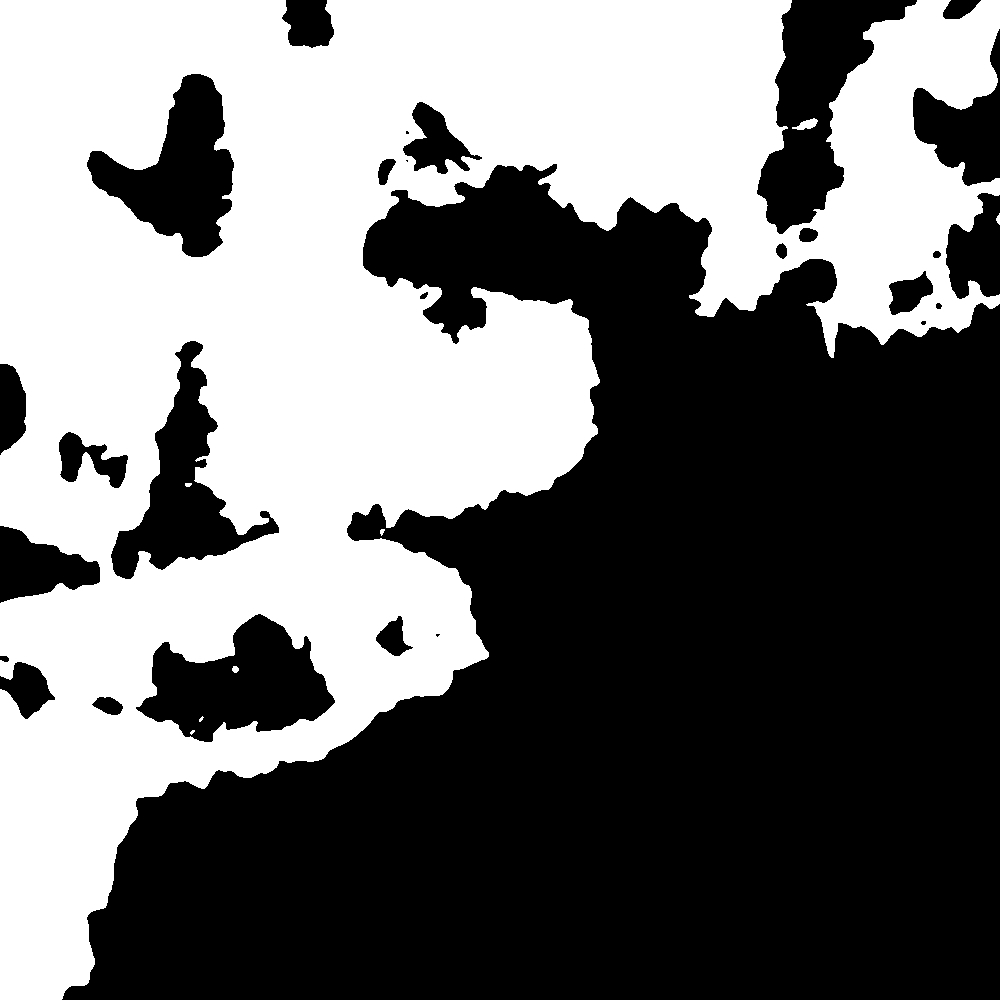
\includegraphics[width=0.23\textwidth]{graphics/aerial06-trav.jpg}
\label{fig:results-trav-06}
}
\subfloat[TFCN output]{
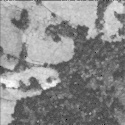
\includegraphics[width=0.23\textwidth]{graphics/tfcn-output-06.jpg}
\label{fig:results-output-06}
}
\caption{Results from cross-validation step 6}
\label{fig:results-06}
\end{figure*}

\begin{figure*}[ht]
\centering
\subfloat[Training and validation losses]{
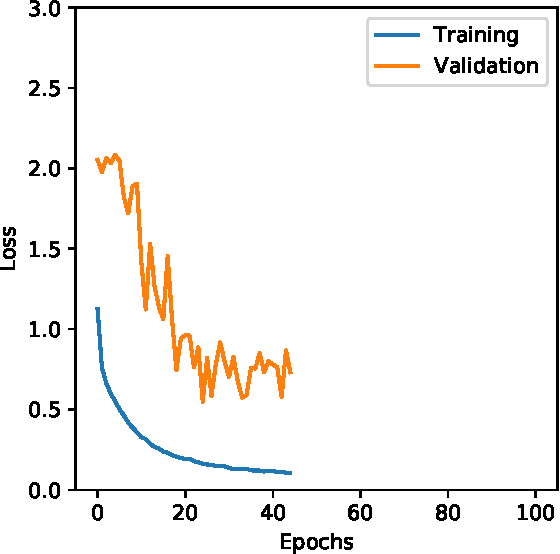
\includegraphics[width=0.23\textwidth]{graphics/loss07.pdf}
\label{fig:results-loss-07}
}
\subfloat[Test image]{
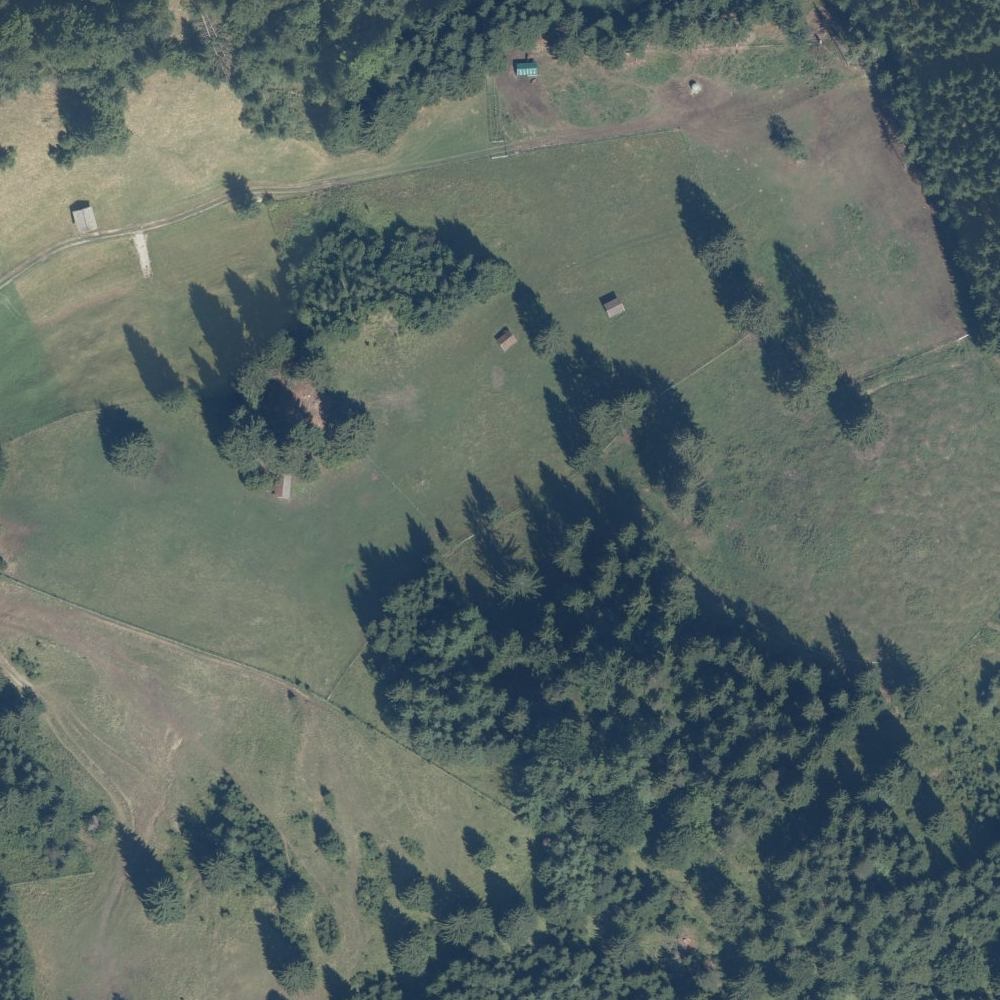
\includegraphics[width=0.23\textwidth]{graphics/aerial07.jpg}
\label{fig:results-input-07}
}
\subfloat[Test label]{
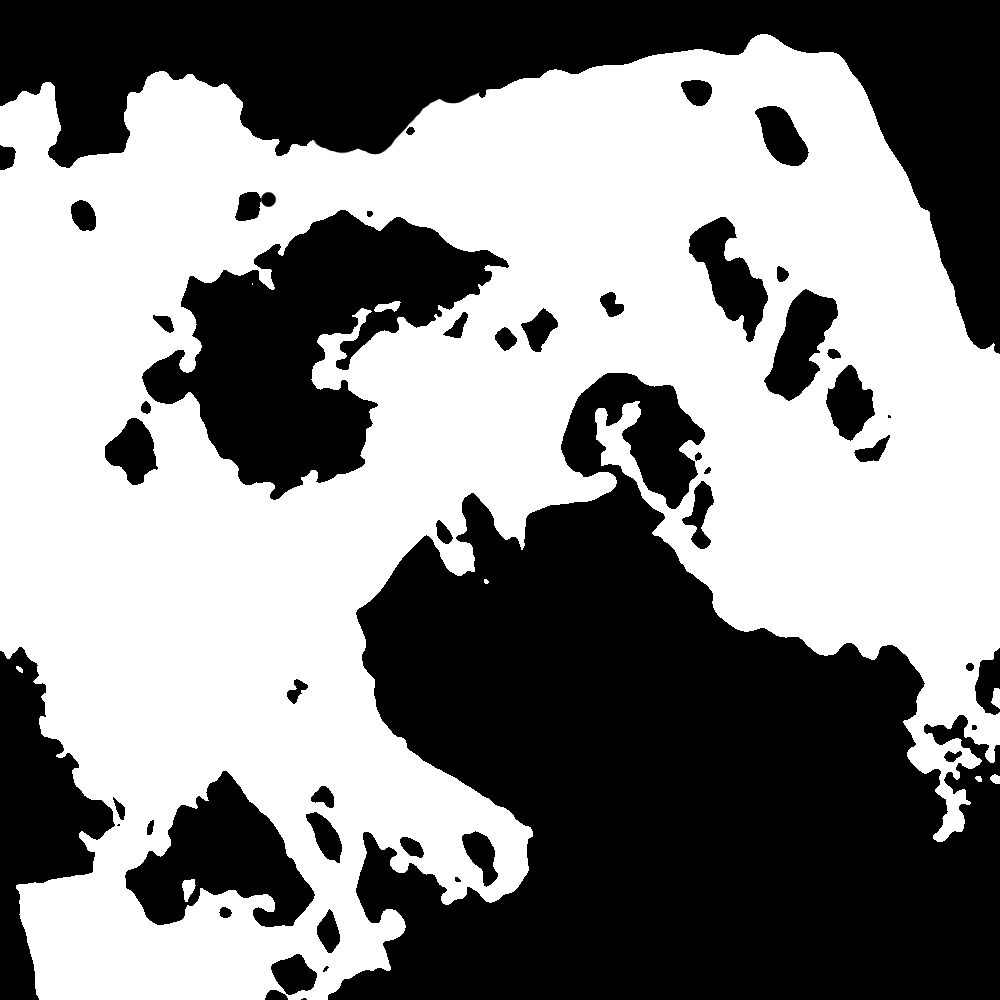
\includegraphics[width=0.23\textwidth]{graphics/aerial07-trav.jpg}
\label{fig:results-trav-07}
}
\subfloat[TFCN output]{
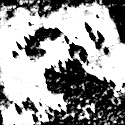
\includegraphics[width=0.23\textwidth]{graphics/tfcn-output-07.jpg}
\label{fig:results-output-07}
}
\caption{Results from cross-validation step 7}
\label{fig:results-07}
\end{figure*}

\begin{figure*}[ht]
\centering
\subfloat[Training and validation losses]{
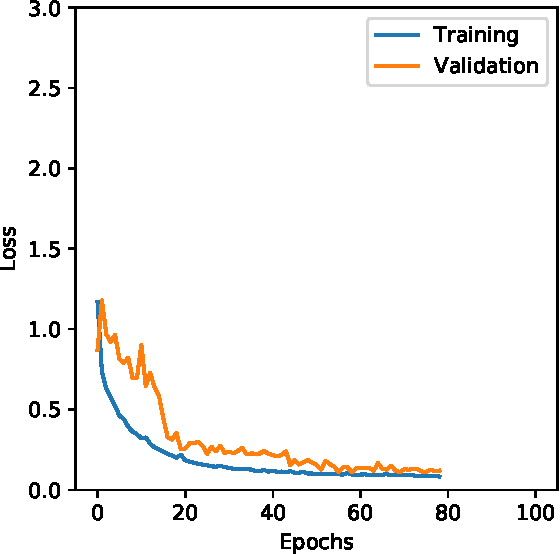
\includegraphics[width=0.23\textwidth]{graphics/loss08.pdf}
\label{fig:results-loss-08}
}
\subfloat[Test image]{
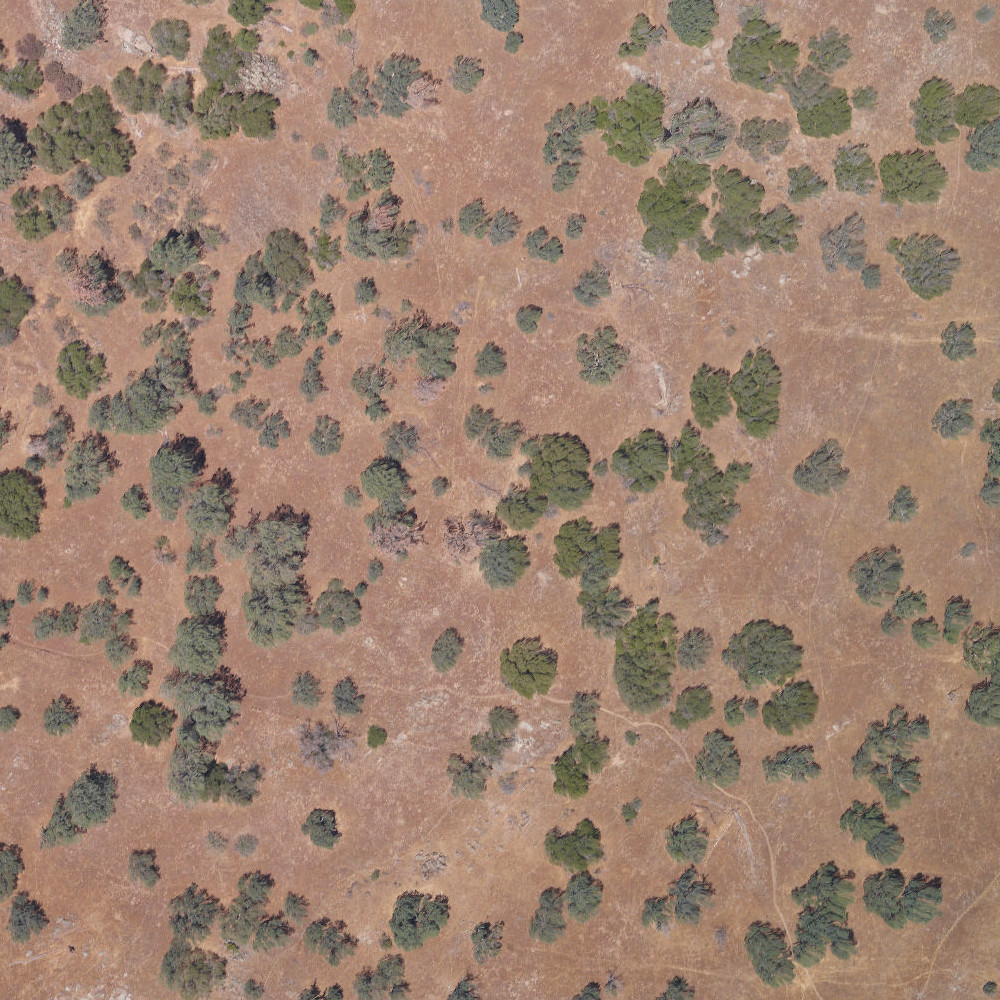
\includegraphics[width=0.23\textwidth]{graphics/aerial08.jpg}
\label{fig:results-input-08}
}
\subfloat[Test label]{
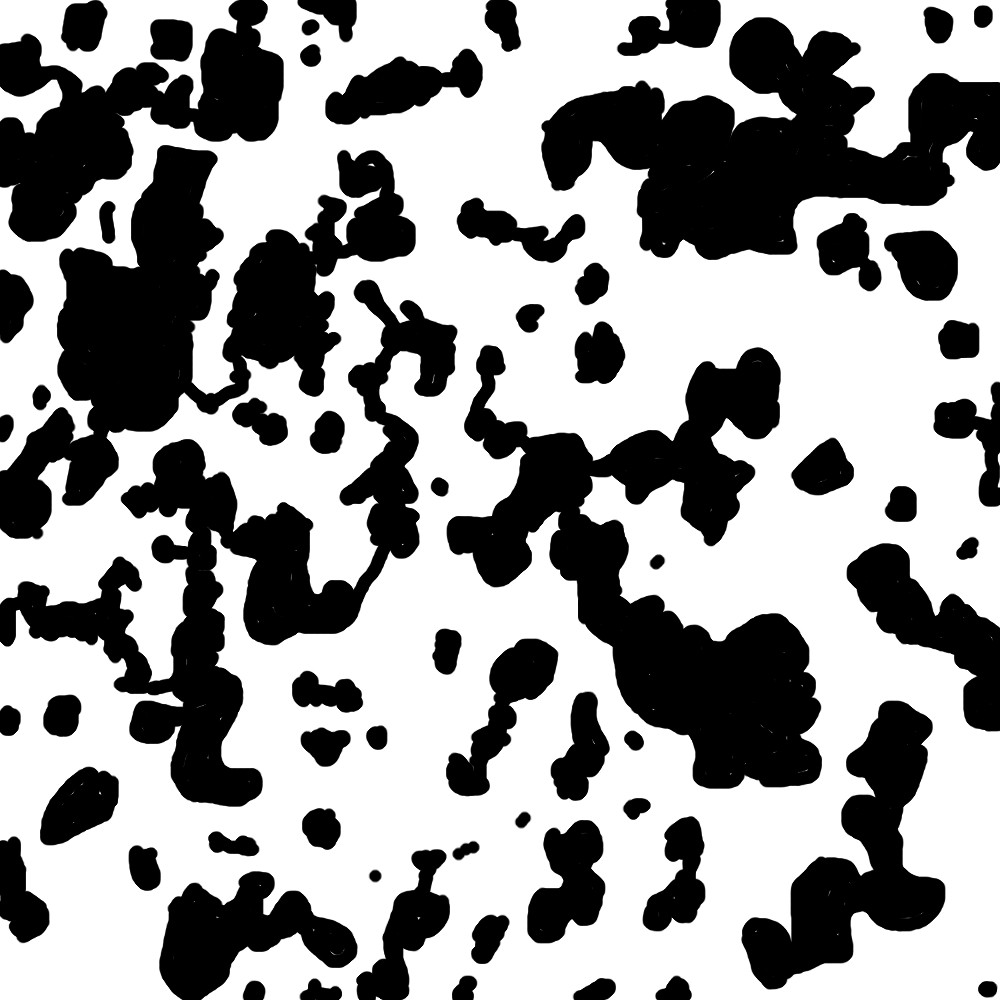
\includegraphics[width=0.23\textwidth]{graphics/aerial08-trav.jpg}
\label{fig:results-trav-08}
}
\subfloat[TFCN output]{
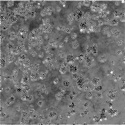
\includegraphics[width=0.23\textwidth]{graphics/tfcn-output-08.jpg}
\label{fig:results-output-08}
}
\caption{Results from cross-validation step 8}
\label{fig:results-08}
\end{figure*}

\section{Discussion}
\label{section:discussion}

It can be seen in Figs. \ref{fig:results-01} through \ref{fig:results-07} that the TFCN outputs closely resemble their corresponding ground truth labels.
This is supported by their relatively low test loss values in Table \ref{tab:results}.
Besides, a number of issues can be observed in the traversability maps.
For example, in the output of Fig. \ref{fig:results-01}, some road patches were marked as not traversable, making it difficult to find shortest paths that might go through these sub-regions.
In Fig. \ref{fig:results-02}, roofs were set as traversable, possibly because their colors and textures look almost the same as the roads'.
The power cables and trails in Fig. \ref{fig:results-03} were given low traversabilities, even though they do not represent real obstacles for a ground robot.
Despite the admirable global performance of the TFCN, these small failures can be significant when applying the model in a real scenario.
Further research is needed to discover how to deal with these issues without compromising the overall achievement.

A larger problem, however, can be identified in Fig. \ref{fig:results-08}, in which there is an attempt to compute the traversability of image 8 from ATPD.
In this case, the TFCN provided a bad traversability estimate.
The test loss for this image was significantly higher.
An hypothesis to explain this behavior relies on the fact that image 8 is remarkably different from the others with respect to terrain type.
Image 8 portrays a sandy landscape with scattered vegetation, however, sandy terrain is not present in other ATPD images.
Since the TFCN had no training with this kind of terrain, the performance of the model on image 8 was degraded.
This problem also highlights that the TFCN is relying heavily on color information to compute its output, since a strong change in color between the training and test sets produced such a negative impact on performance.
A possible advance would be to find a method to weight the influence of color and texture in the inner-workings of the TFCN and improve its generalization capabilities.

\begin{table}[htbp]
\begin{center}
\caption{MSE comparison}
\begin{tabular}{|c|c c|}
\hline
\textbf{Input Image} & \textbf{Borges et al.\cite{borges:2019}} & \textbf{TFCN} \\
% \cline{2-4}
\textbf{ATPD ID} & \textbf{MSE} & \textbf{MSE} \\
\hline
1 & 0.1566 & \cellcolor{blue!15} 0.1245 \\ %\hline
2 & 0.2066 & \cellcolor{blue!15} 0.1177 \\ %\hline
3 & 0.1714 & \cellcolor{blue!15} 0.1137 \\ %\hline
4 & 0.1265 & \cellcolor{blue!15} 0.0986 \\ %\hline
5 & 0.1394 & \cellcolor{blue!15} 0.0688 \\ %\hline
6 & 0.1420 & \cellcolor{blue!15} 0.0796 \\ %\hline
7 & \cellcolor{blue!15} 0.1756 & 0.2279 \\ %\hline
8 & \cellcolor{blue!15} 0.1488 & 0.5114 \\ \hline
\end{tabular}
\label{tab:comparison-mse}
\end{center}
\end{table}

A comparison was made to evaluate the TFCN results relative to previous work about traversability based on aerial images.
This comparison required a quantitative measurement of the quality of traversability outputs, either by an accuracy or error estimate over a test set.
At the time of writing, only one work \cite{borges:2019} could be reproduced and tested for this comparison.
Table \ref{tab:comparison-mse} contains the MSE between the test labels and the model outputs for all images in ATPD.
The TFCN surpassed \cite{borges:2019} in almost all cases (1 through 6) by a significant margin.
In cases 7 and 8, however, it was surmounted.
For image 8, the cause is clear: it has been seen before that this image was a challenge to the TFCN, given the lack of training data in sandy terrain.
For image 7, a good hypothesis to account for the unusually high MSE is that in this specific leave-one-out step, image 8 was used for validation and, for the same reason mentioned before, it disrupted the training process.
The overall MSE comparison shows that the TFCN overcomes the mentioned competitor with respect to quality of traversability outputs.
However, further research is needed to fix the observed generalization issue.


To analyze the TFCN with regard to processing time, two papers were selected.
The works by Hudjakov and Tamre \cite{hudjakov:2013} and Borges et al. \cite{borges:2019} were chosen because they clearly state the processing times achieved by their models.
Moreover, \cite{hudjakov:2013} also uses CNNs to compute traversabilities, making it a good candidate for comparison and validation of a new CNN architecture.
The processing times in Table \ref{tab:comparison-time} regarding the work by H \& T were extracted directly from the paper, in which the authors compute traversability maps over images of $2000 \times 2000$ pixels.
The values for images of $1000 \times 1000$ pixels were extrapolated from information about total patterns in the image and number of patterns classified per second, as stated in the paper.
The remaining processing times were obtained from implementations of the models.
It is clear from Table \ref{tab:comparison-time} that the TFCN greatly reduces processing times when compared with \cite{hudjakov:2013}, even when running on less powerful hardware.
The reason for this large advantage is that the TFCN generates the entire traversability map in only one forward pass through the network, while the CNN model proposed by H \& T needs to perform classification on millions of overlapping patterns to produce a single map.
The TFCN also outperforms \cite{borges:2019} by a narrower margin.
This difference, however, could greatly increase if the input images were larger.


\begin{table}[htbp]
\begin{center}
\caption{TIME comparison}
\begin{tabular}{|c|c c c|}
\hline
\textbf{Input Image} & \textbf{H. \& T. \cite{hudjakov:2013}} & \textbf{Borges et al.\cite{borges:2019}} & \textbf{TFCN} \\
% \cline{2-4}
\textbf{Size} & \textbf{Time (s)} & \textbf{Time (s)} & \textbf{Time (s)} \\
\hline
$1000 \times 1000$ & 1250 \ $^{b*}$  \ \ \ 11 \ $^{c*}$ & 0.834 \ $^{a\ }$ & \cellcolor{blue!15} 0.775 \ $^{a}$ \\ %\hline
$2000 \times 2000$ & 5000 \ $^{b\phantom{*}}$  \ \ \ 44 \ $^{c\ }$ & 3.336 \ $^{a*}$ & \cellcolor{blue!15} 2.583 \ $^{a}$ \\ \hline
\end{tabular} \\[0.01cm]
\label{tab:comparison-time}
\end{center}
\hspace{0.2cm}
\begin{minipage}[t]{\textwidth}
\scriptsize{a. Intel Core i5 650 CPU} \\
\scriptsize{b. Intel Core i7 920 CPU} \\
\scriptsize{c. 2x Nvidia GTX 570 GPUs} \\
\scriptsize{* Estimate based on number of patterns per image and processing speed}
\end{minipage}
\end{table}

\section{Conclusion}
\label{section:conclusion}

This work proposed TFCN, a new fully convolutional neural network model to compute traversabilities from aerial images with the purpose of helping ground robot navigation.
The TFCN was trained on the Aerial Traversability and Planning Dataset and cross-validated using an image-based leave-one-out approach.
The results showed that the TFCN outperformed its competitors with regard to quality of traversability outputs, as measured with MSE against ground-truths, and processing time.
However, it was shown that the current implementation of the TFCN has a generalization issue when it comes to terrain type.
Further research is needed to address this issue.

\bibliography{references}
\bibliographystyle{ieeetr}

% \begin{thebibliography}{00}
% \bibitem{b1} G. Eason, B. Noble, and I. N. Sneddon, ``On certain integrals of Lipschitz-Hankel type involving products of Bessel functions,'' Phil. Trans. Roy. Soc. London, vol. A247, pp. 529--551, April 1955.
% \bibitem{b2} J. Clerk Maxwell, A Treatise on Electricity and Magnetism, 3rd ed., vol. 2. Oxford: Clarendon, 1892, pp.68--73.
% \bibitem{b3} I. S. Jacobs and C. P. Bean, ``Fine particles, thin films and exchange anisotropy,'' in Magnetism, vol. III, G. T. Rado and H. Suhl, Eds. New York: Academic, 1963, pp. 271--350.
% \bibitem{b4} K. Elissa, ``Title of paper if known,'' unpublished.
% \bibitem{b5} R. Nicole, ``Title of paper with only first word capitalized,'' J. Name Stand. Abbrev., in press.
% \bibitem{b6} Y. Yorozu, M. Hirano, K. Oka, and Y. Tagawa, ``Electron spectroscopy studies on magneto-optical media and plastic substrate interface,'' IEEE Transl. J. Magn. Japan, vol. 2, pp. 740--741, August 1987 [Digests 9th Annual Conf. Magnetics Japan, p. 301, 1982].
% \bibitem{b7} M. Young, The Technical Writer's Handbook. Mill Valley, CA: University Science, 1989.
% \end{thebibliography}

\end{document}
